\documentclass{article}

% packages
\usepackage{amsmath, amsthm, thmtools, amsfonts, amssymb, luacode, catchfile, tikzducks, hyperref, ifthen}
\ifcsname c@kobocompile\endcsname
	\usepackage[a5paper, total={1072pt, 1448pt}, margin=10pt, includeheadfoot]{geometry} % set page margins
\else
	\usepackage[a4paper, margin=50pt, includeheadfoot]{geometry}
\fi
\usepackage[shortlabels]{enumitem}
\usepackage[skip=3pt, indent=0pt]{parskip}

% language
\usepackage[bidi=basic, layout=tabular, provide=*]{babel}
\ifcsname c@english\endcsname
	\babelprovide[main, import]{english}
\else
	\babelprovide[main, import]{hebrew}
	\babelprovide{rl}
\fi
%\babelfont{rm}{Libertinus Serif}
\babelfont{rm}[Renderer=Harfbuzz]{Libertinus Serif}
\babelfont{sf}{Libertinus Sans}
\babelfont{tt}{Libertinus Mono}

% style
\AddToHook{cmd/section/before}{\clearpage}	% Add line break before section
\linespread{1.3}
\setcounter{secnumdepth}{0}		% Remove default number tags from sections, this won't do well with theorems
\AtBeginDocument{\setlength{\belowdisplayskip}{3pt}}
\AtBeginDocument{\setlength{\abovedisplayskip}{3pt}}
\graphicspath{ {../images/} }

% operators
\DeclareMathOperator\cis{cis}
\DeclareMathOperator\Sp{Sp}
\DeclareMathOperator\tr{tr}
\DeclareMathOperator\im{Im}
\DeclareMathOperator\re{Re}
\DeclareMathOperator\diag{diag}
\DeclareMathOperator*\lowlim{\underline{lim}}
\DeclareMathOperator*\uplim{\overline{lim}}
\DeclareMathOperator\rng{rng}
\DeclareMathOperator\Sym{Sym}
\DeclareMathOperator\Arg{Arg}
\DeclareMathOperator\Log{Log}
\DeclareMathOperator\dom{dom}
\DeclareMathOperator\supp{Supp}
\DeclareMathOperator\var{Var}
\DeclareMathOperator\cov{Cov}

% commands
%\renewcommand\qedsymbol{\textbf{מש''ל}}
%\renewcommand\qedsymbol{\fbox{\emoji{lizard}}}
\newcommand{\Aa}[0]{\mathcal{A}}
\newcommand{\Bb}[0]{\mathcal{B}}
\newcommand{\CC}[0]{\mathbb{C}}
\newcommand{\Cc}[0]{\mathcal{C}}
\newcommand{\EE}[0]{\mathbb{E}}
\newcommand{\FF}[0]{\mathbb{F}}
\newcommand{\Ff}[0]{\mathcal{F}}
\newcommand{\Ii}[0]{\mathcal{I}}
\newcommand{\Gg}[0]{\mathcal{G}}
\newcommand{\Ll}[0]{\mathcal{L}}
\newcommand{\Mm}[0]{\mathcal{M}}
\newcommand{\NN}[0]{\mathbb{N}}
\newcommand{\Nn}[0]{\mathcal{N}}
\newcommand{\PP}[0]{\mathbb{P}}
\newcommand{\Pp}[0]{\mathcal{P}}
\newcommand{\QQ}[0]{\mathbb{Q}}
\newcommand{\RR}[0]{\mathbb{R}}
\newcommand{\Rr}[0]{\mathcal{R}}
\newcommand{\Ss}[0]{\mathcal{S}}
\newcommand{\TT}[0]{\mathbb{T}}
\newcommand{\Uu}[0]{\mathcal{U}}
\newcommand{\Vv}[0]{\mathcal{V}}
\newcommand{\Ww}[0]{\mathcal{W}}
\newcommand{\ZZ}[0]{\mathbb{Z}}
\newcommand{\acts}[0]{\circlearrowright}
\newcommand{\explain}[2] {
	\begin{flalign*}
		 && \text{#2} && \text{#1}
	\end{flalign*}
}
\newcommand{\maketitleprint}[0]{ \begin{center}
	%\begin{tikzpicture}[scale=3]
	%	\duck[graduate=gray!20!black, tassel=red!70!black]
	%\end{tikzpicture}	
	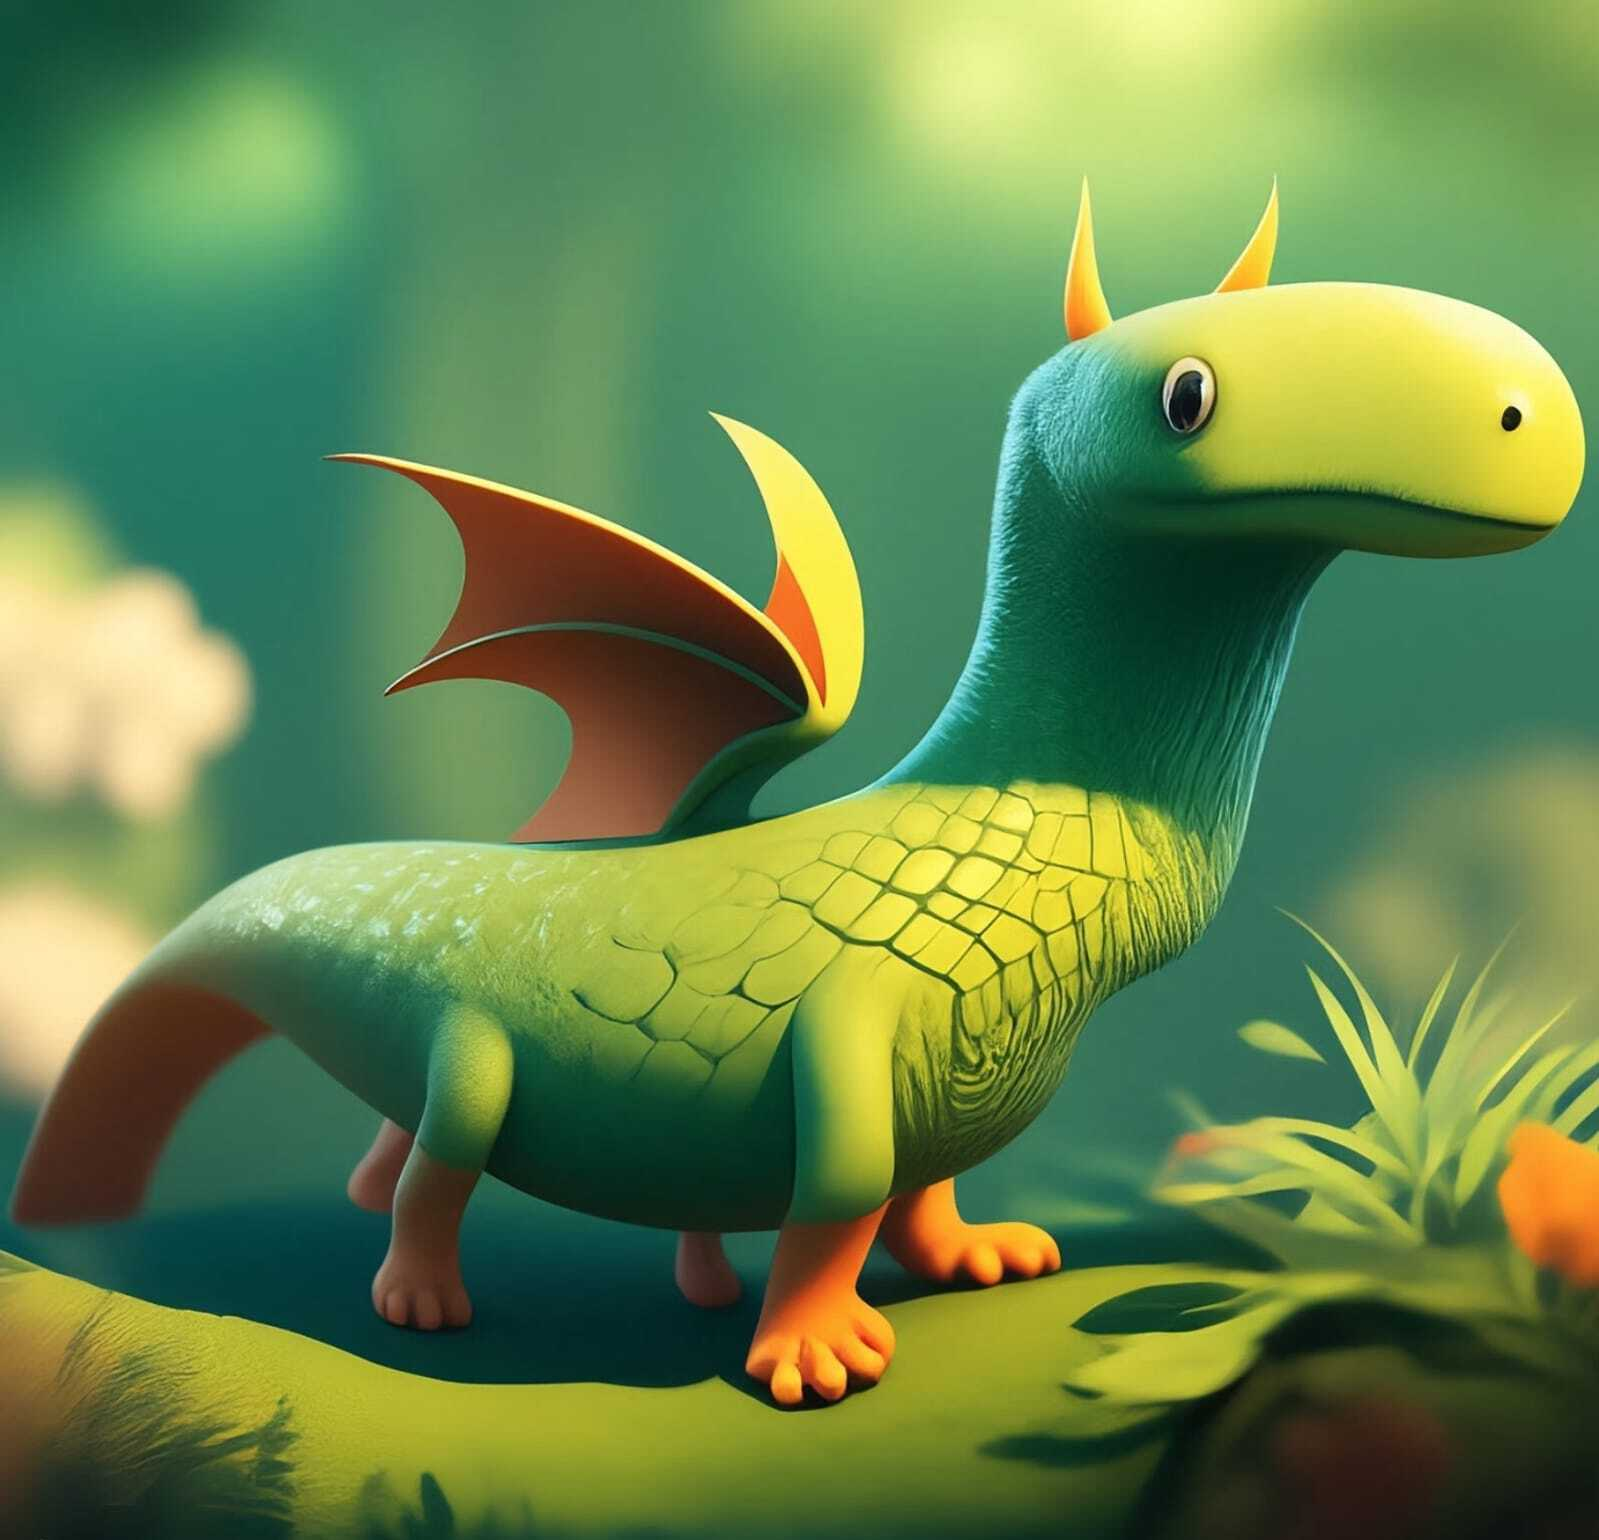
\includegraphics[width=6cm]{cover}
\end{center}
}

% theorem commands
\newtheoremstyle{c_remark}
	{}	% Space above
	{}	% Space below
	{}% Body font
	{}	% Indent amount
	{\bfseries}	% Theorem head font
	{}	% Punctuation after theorem head
	{.5em}	% Space after theorem head
	{\thmname{#1}\thmnumber{ #2}\thmnote{ \normalfont{\text{(#3)}}}}	% head content
\newtheoremstyle{c_definition}
	{3pt}	% Space above
	{3pt}	% Space below
	{}% Body font
	{}	% Indent amount
	{\bfseries}	% Theorem head font
	{}	% Punctuation after theorem head
	{.5em}	% Space after theorem head
	{\thmname{#1}\thmnumber{ #2}\thmnote{ \normalfont{\text{(#3)}}}}	% head content
\newtheoremstyle{c_plain}
	{3pt}	% Space above
	{3pt}	% Space below
	{\itshape}% Body font
	{}	% Indent amount
	{\bfseries}	% Theorem head font
	{}	% Punctuation after theorem head
	{.5em}	% Space after theorem head
	{\thmname{#1}\thmnumber{ #2}\thmnote{ \text{(#3)}}}	% head content

\ifcsname c@english\endcsname
	\theoremstyle{plain}
	\newtheorem{theorem}{Theorem}[section]
	\newtheorem{lemma}[theorem]{Lemma}
	\newtheorem{proposition}[theorem]{Proposition}
	\newtheorem*{proposition*}{Proposition}
	%\newtheorem{corollary}[theorem]{אין חלופה עברית}

	\theoremstyle{definition}
	\newtheorem{definition}[theorem]{Definition}
	\newtheorem*{definition*}{Definition}
	\newtheorem{example}{Example}[section]
	\newtheorem{exercise}{Exercise}[section]

	\theoremstyle{remark}
	\newtheorem*{remark}{Remark}
	\newtheorem*{solution}{Solution}
	\newtheorem{conclusion}[theorem]{Conclusion}
	\newtheorem{notation}[theorem]{Notation}
\else
	\theoremstyle{c_plain}
	\newtheorem{theorem}{משפט}[section]
	\newtheorem{lemma}[theorem]{למה}
	\newtheorem{proposition}[theorem]{טענה}
	\newtheorem*{proposition*}{טענה}
	%\newtheorem{corollary}[theorem]{אין חלופה עברית}

	\theoremstyle{c_definition}
	\newtheorem{definition}[theorem]{הגדרה}
	\newtheorem*{definition*}{הגדרה}
	\newtheorem{example}{דוגמה}[section]
	\newtheorem{exercise}{תרגיל}[section]

	\theoremstyle{c_remark}
	\newtheorem*{remark}{הערה}
	\newtheorem*{solution}{פתרון}
	\newtheorem{conclusion}[theorem]{מסקנה}
	\newtheorem{notation}[theorem]{סימון}
\fi

% Questions related commands
\newcounter{question}
\setcounter{question}{1}
\newcounter{sub_question}
\setcounter{sub_question}{1}

\ifcsname c@english\endcsname
	\newcommand{\question}[1][0]{
		\ifthenelse{#1 = 0}{}{\setcounter{question}{#1}}
		\section{Question \arabic{question}}
		\addtocounter{question}{1}
		\setcounter{sub_question}{1}
	}

	\newcommand{\subquestion}[1][0]{
		\ifthenelse{#1 = 0}{}{\setcounter{sub_question}{#1}}
		\subsection{Part \alph{sub_question}}
		\addtocounter{sub_question}{1}
	}
\else
	\newcommand{\question}[1][0]{
		\ifthenelse{#1 = 0}{}{\setcounter{question}{#1}}
		\section{שאלה \arabic{question}}
		\addtocounter{question}{1}
		\setcounter{sub_question}{1}
	}

	\newcommand{\subquestion}[1][0]{
		\ifthenelse{#1 = 0}{}{\setcounter{sub_question}{#1}}
		\subsection{סעיף \localecounter{letters.gershayim}{sub_question}}
		\addtocounter{sub_question}{1}
	}
\fi

% import lua and start of document
\directlua{common = require ('../common')}

\GetEnv{AUTHOR}

% headers
\author{\AUTHOR}
\date\today

\title{פתרון מטלה 05 --- תורת הקבוצות (80200)}

\begin{document}
\maketitle
\maketitleprint{}

\directlua{ Q_number = 3 }
\Question{}
תהי $\langle A, \le \rangle$ קבוצה סדורה חלקית.

\Subquestion{}
תהי $B \subseteq A$, ונוכיח כי $\langle B, \le \cap (B \times B) \rangle$ היא קבוצה סדורה חלקית אף היא.
\begin{proof}
	נבדוק את תכונות הסדר החלקי.
	\begin{enumerate}
		\item טרנזיטיביות: $\langle a, b \rangle, \langle b, c \rangle \in \le \cap B^2 \implies a \le c \land a, c \in B \implies (a, c) \in \le \cap B^2$.
		\item רפלקסיביות: $\forall b \in B : \langle b, b \rangle \in \le \land \langle b, b \rangle \in B^2 \implies \langle b, b \rangle \in (\le \cap B^2)$.
		\item אנטי־סימטריה: $\forall a, b \in B : \langle a, b \rangle, \langle b, a \rangle \in (\le \cap B^2) \implies a = b, b \in B$
	\end{enumerate}
	ומצאנו כי כל ההגדרות מתקיימות.
\end{proof}

\Subquestion{}
נוכיח כי אם $a \in A$ הוא מינימום, אז הוא איבר מינימלי והמינימלי היחיד.
\begin{proof}
	נניח כי $a \in A$ הוא מינימום ולכן $\forall b \in A : a \le b$. \\*
	יהי איבר $b \in A$ המקיים $b \le a$, אבל ידוע כי $a \le b$ ולכן נסיק מהאנטי־סימטריה כי $a = b$, ולכן נובע כי $a$ איבר מינימלי. \\*
	נניח כי קיים איבר $b \in A$ אשר הוא מינימלי, ואנו יודעים כי $a \le b$, ולכן נובע מהמינימליות כי $a = b$, ומצאנו כי קיים איבר מינימלי יחיד והוא $a$.
\end{proof}

\Subquestion{}
נוכיח כי הכיוון ההפוך לטענה הקודמת איננו נכון, קיום מינימלי יחיד לא גורר כי קיים מינימום.
\begin{proof}
	נבחן את $\langle \ZZ, \le \rangle$ כאשר מוציאים את כל הזוגות הסדורים שמעורבים ב־$0$, מלבד $\langle 0, 0 \rangle$. \\*
	סדר זה עומד בכלל ההגדרות, אין מינימום או מקסימום, ואפס הוא מינימלי.
\end{proof}

\Subquestion{}
נוכיח שאם $\langle A, \le \rangle$ הוא סדר מלא אז איבר הוא מינימלי אם ורק אם הוא המינימום.
\begin{proof}
	\textbf{כיוון ראשון:}
	נניח כי $a \in A$ הוא איבר מינימילי. לכן $\forall b \in a : b \le a \implies a = b$. \\*
	כל איבר $b \in A$ מקיים $b \le a \implies a = b \implies a \le b$ או $a \le b$ ולכן נקבל כי $a \le b$ בכל מקרה, ולכן $a$ מינימום.

	\textbf{כיוון שני:}
	נניח כי $a$ הוא מינימום ולכן $\forall b \in A : a \le b$. \\*
	יהי $b \in A, b \le a$, אז $a \le b$ ובפרט $a = b$ וקיבלנו כי גם הגדרת המינימלי חלה.
\end{proof}

\Subquestion{}
נוכיח כי אם $A$ סופית ולא ריקה אז יש בה איבר מינימלי.
\begin{proof}
	נניח בשלילה כי לא קיים איבר מינימלי, לכן $\forall a \in A \exists b \in A : b \le a, a \ne b$. \\*
	נניח ש־$|A| = n$ ונבחר $a_1 \in A$, כלשהו, נגדיר $a_2 \le a_1, a_1 \ne a_2$, ובאופן דומה נגדיר $a_{k + 1} \le a_k, a_{k + 1} \ne a_k$. \\*
	נבנה כך סדרה באורך $n + 1$ ונסיק מעיקרון שובך היונים שאיבר כלשהו $a_k$ מופיע פעמיים בסדרה ומקיים $a_k \le a_k, a_k \ne a_k$ בסתירה להנחתנו כי אין איבר מינימלי.
\end{proof}

\Question{}
יהיו ארבעה יחסים מעל $\NN^\NN$:
\begin{align*}
	& R_1 = \{ \langle f, g \rangle \in \NN^\NN \times \NN^\NN \mid \forall m : f(m) \le g(m) \} \\
	& R_2 = \{ \langle f, g \rangle \in \NN^\NN \times \NN^\NN \mid \exists n \forall m : m > n \implies f(m) \le g(m) \} \\
	& R_3 = \{ \langle f, g \rangle \in \NN^\NN \times \NN^\NN \mid \forall n \exists m, m > n \implies f(m) \le g(m) \} \\
	& R_4 = \{ \langle f, g \rangle \in \NN^\NN \times \NN^\NN \mid f = g \lor (\exists n : f \restriction [n] = g \restriction [n] \land f(n) < g(n)) \}
\end{align*}

\Subquestion{}
נבדוק עבור כל יחס אם הוא רפלקסיבי, טרנזיטיבי ואנטי־סימטרי.

עבור $R_1$:
\begin{enumerate}
	\item נשים לב כי בהינתן $f \in \NN^\NN$ לכל $m \in \NN$ נקבל $f(m) = f(m) \implies f(m) \le f(m)$ ולכן $R_1$ הוא רפלקסיבי.
	\item יהיו $f R_1 g, g R_1 h$ ויהי $m \in \NN$, אז $f(m) \le g(m), g(m) \le h(m)$ ולכן גם $f(m) \le h(m)$ ולכן $f R_1 h$, והיחס טרנזיטיבי.
	\item יהיו $f R_1 g$ כך שגם $g R_1 f$ אז לכל $m \in \NN$ אז $f(m) \le g(m)$ וגם $g(m) \le f(m)$ ולכן נוכל להסיק $f(m) = g(m)$, דהינו $f = g$, ולכן היחס אנטי־סימטרי.
\end{enumerate}
עבור $R_2$:
\begin{enumerate}
	\item נוכל להניח כי רפלקסיביות מתקיימת שכן אם נבחר $m = 0$ נקבל את התנאי של רפלקסיביות עבור $R_1$.
	\item יהיו $f R_2 g, g R_2 h$, לכן קיימים $n_1, n_2$ כך שבהתאמה לכל $m > n_1, n_2$ מתקיים $f(m) = g(m), g(m) = h(m)$, ולכן נבחר $n = \max\{n_1, n_2\}$ ועבורו לכל $m > n$ נקבל $f(m) \le g(m) \le h(m)$ ולכן $g R_2 h$.
	\item נניח כי $f R_2 g, g R_2 f$, ונבחר באופן דומה להוכחת הסימטריה $n$ מינימלי עבורו $m > n > 0$ מקיים $f(m) = g(m)$, אבל עבור $m = 0$ יכול להיות ש־$f(m) \ne g(m)$ ולכן לא מתקיימת אנטי־סימטריה.
\end{enumerate}
עבור $R_3$:
\begin{enumerate}
	\item לכל $f$ ולכל $n \in \NN$ מתקיים $f(n) = f(n)$ ולכן נוכל לבחור $m = n + 1$ לכל $n$ ונקבל כי $f R_3 f$, דהינו היחס הוא רפלקסיבי.
	\item נגדיר פונקציות הבנויות ממחזור המספרים הבא $f = (3, 2, 3, 3, 3, \dots), g = (2, 2, 3, 2, 2, \dots), h = (1, 1, 1, 2, 1, \dots)$, מאופן הבנייה נובע כי $f R_3 g, g R_3 h$ אבל לכל $m \in \NN$ גם $f(m) > h(m)$. \\*
		לכן נסיק כי היחס לא טרנזיטיבי.
	\item נגדיר
		\[
			f(m) = \begin{cases}
				1 & m \in 2\NN \\
				0 & m \notin 2\NN
			\end{cases},
			g(m) = 1 - f(m)
		\]
		נבחין כי $f R_3 g, g R_3 f$, אבל $f \ne g$, ולכן היחס לא אנטי־סימטרי.
\end{enumerate}
עבור $R_4$:
\begin{enumerate}
	\item היחס מוגדר להיות רפלקסיבי.
	\item יהיו $f R_4 g, g R_4 h$, אז קיים $n_1, n_2$ המקיימים את תנאי ההגדרה של הקבוצה עבור $f, g$ ו־$g, h$ בהתאמה. \\*
		נבחר $n = \min\{ n_1, n_2 \}$ ונקבל כי $\forall m < n : f(m) = g(m) = h(m)$, ועבור $m = n$ נקבל כי $f(m) < g(m) = h(m)$ או $f(m) = g(m) < h(m)$ ובכל מקרה קיבלנו כי $f(m) < h(m)$ וקיבלנו כי טרנזיטיביות חלה.
	\item נבחין כי אם $f R_4 g$ וגם $g R_4 f$ מדרך ההוכחה של הסעיף הקודם נקבל כי $f(m) \ne f(m)$ עבור $m$ כלשהו ולכן נסיק ש־$f = g$ כמתקבל מהתנאי הראשון של הגדרת הקבוצה.
\end{enumerate}

\Subquestion{}
מצאנו כי $R_1, R_4$ הם סדרים.

\subsubsection{i.}
נוכיח כי $R_1$ איננו יחס קוווי ואילו כי $R_4$ הוא אכן יחס קווי.
\begin{proof}
	עבור $R_1$ מספיק שנציג דוגמה נגדית, ולכן נבחר את הדוגמה ל־$f, g$ מהסתירה כי $R_3$ היא אנטי־סימטרית. \\*
	ראינו כי $g(0) \le g(0)$ אבל $g(1) \not\le f(1)$ וגם כי $f(1) \le g(1)$ אבל $f(0) \not\le g(0)$ ולכן $\langle f, g \rangle \notin R_1, \langle g, f \rangle \notin R_1, f \ne g$ וקיבלנו כי היחס לא קווי.

	נוכיח כי $R_4$ הוא אכן קווי. \\*
	הגדרתו מכילה איברים שווים ולכן מספיק שנוכיח כי אם $f \ne g$ אז או $f R_4 g$ או $g R_4 f$ בלבד. \\*
	יהיו $f, g \in \NN^\NN$ כך ש־$f \ne g$ וגדיר $n \in \NN$ המספר המקסימלי עבורו $\forall m \in \NN, m < n : f(m) = g(m)$. \\*
	נבחין כי יתכן ש־$n = 0$ והטענה הזו מתקיימת באופן ריק בלבד. 
	מאיך שהגדרנו את $n$ נקבל כי $f(n) \ne g(n)$, ולכן או ש־$f(n) < g(n)$ ונגרר כי $f R_4 g$ או ש־$g(n) < f(n)$ ומתקבל $g R_4 f$ בלבד.
\end{proof}

\subsubsection{ii.}
נבדוק את קיומם של איברים מינימליים, מקסימליים ואת קיומו של מינימום ומקסימום.

נבחן תחילה את $R_1$, ונטען ש־$f$ המוגדרת על־ידי $f(n) = 0$ היא המינימום. \\*
לכל פונקציה $g$ שנבחר ולכל $m \in \NN$ נקבל $f(m) = 0 \le g(m)$ ולכן מצאנו כי זהו המינימום, ולכן מטענה מהשאלה הקודמת נקבל כי זהו גם האיבר המינימלי היחיד. \\*
נבחר פונקציה כלשהי $f$, ונגדיר $g$ על־ידי $g(n) = f(n) + 1$, ולכן מהגדרת $R_1$ נסיק כי $f R_1 g$. \\*
לכן מצאנו כי לכל פונקציה קיימת פונקציה גדולה ממנה ולכן אין איבר מקסימלי או מקסימום.

נעבור עתה ל־$R_4$. זהו יחס קווי ולכן כפי שהוכחנו אם יש איבר מינימום אז הוא המינימלי היחד. \\*
גם הפעם נבחר את $f(n) = $, ונבחין כי לכל פונקציה או שמתקיים $g(n) = 0$ ולכן $g = f$ או ש־$g \ne f$ ולכן קיים $m$ עבורו $g(m) > 0$ ונקבל ישירות $f R_4 g$, דהינו $f$ היא המינימום וההאיבר המינימלי היחיד ביחס. \\*
תהי פונקציה $f$, ונגדיר פונקציה $g$ על־ידי $g(n) = f(n + 1)$, ולכן מתקיים $f(0) < g(1)$ ונקבל כי $f R_4 g$, ולכן אין איבר מקסימלי או מקסימום ביחס.

\Question{}
\Subquestion{}
נוכיח ש־$\trianglelefteq$ הוא יחס סדר חלקי על $Seq(A)$.
\begin{proof}
	נבדוק את הגדרת יחס סדר:
	\begin{enumerate}
		\item רפלקסיביות: יהי $a \in A$, אז $a \trianglelefteq a$ שכן אורך הסדרה זהה לעצמו וכן כלל האיברים שווים.
		\item טרנזיטיביות: יהיו $a \trianglelefteq b, b \trianglelefteq c$, ונגדיר $m_a, m_b, m_c$ אורכי הסדרות,
			אז $m_a \le m_b, m_b \le m_c$ ונקבל $m_a \le m_c$, ולכל $i < m_a$ נקבל $a_i = b_i = c_i$ וקיבלנו כי $a \trianglelefteq c$.
		\item אנטי־סימטריה: נניח כי $a \trianglelefteq b$ וגם $b \trianglelefteq a$, ויהיו $m, n$ אורכי $a, b$ בהתאמה.
			אז נקבל $n \le m, m \le n$ ולכן $m = n$, וגם לכל $i < m$ מתקיים $a_i = b_i$ ולכן $a = b$.
	\end{enumerate}

	נראה על־ידי דוגמה נגדית כי זהו לא יחס מלא, דהינו שהוא חלקי. \\*
	נבחר $a = (1), b = (2)$, אז $a \not\trianglelefteq b$ וגם $b \not\trianglelefteq a$ על־פי ההגדרה, וכמובן $a \ne b$.
\end{proof}

\Subquestion{}
נמצא תנאי מספיק והכרחי ל־$A$ כך ש־$\trianglelefteq$ יהיה יחס סדר מלא על $Seq(A)$.

מצאנו כי היחס לא חל על סדרות שונות מאורך זהה, ולכן מספיק שנגביל את $A$ להיות יחידון ונקבל כי אם $a, b \in Seq(A)$ אז $a \trianglelefteq b$ או $b \trianglelefteq a$ או $a = b$ כמתבקש. \\*
נניח מהצד השני כי שתי סדרות באורך זהה $a, b$ מקיימות $a \trianglelefteq b$ או $b \trianglelefteq$, אז מההגדרה נקבל כי $a = b$ ולכן איבריהם זהים.

\Subquestion{}
נמצא תנאי מספיק והכרחי עבורו יהיה איבר מקסימלי ב־$Seq(A)$. \\*
נניח כי קיים איבר מקסימלי ב־$A$, ונניח בשלילה שאורכו $1$ לפחות, לכן נוכל לבנות סדרה חדשה $b$ על־ידי הכפלת האיבר ונקבל $a \trianglelefteq b$, בסתירה למקסימליות, לכן נסיק שכדי שיהיה איבר מקסימלי הוא צריך להיות מגודל $0$. \\*
דהינו נקבל כי $A = \emptyset$. \\*
מהצד השני נניח כי $A = \emptyset$ ולכן גם $Seq(A) = \{ \emptyset \}$ והקבוצה היא יחידון ולכן ישנו איבר מקסימלי.

\end{document}
